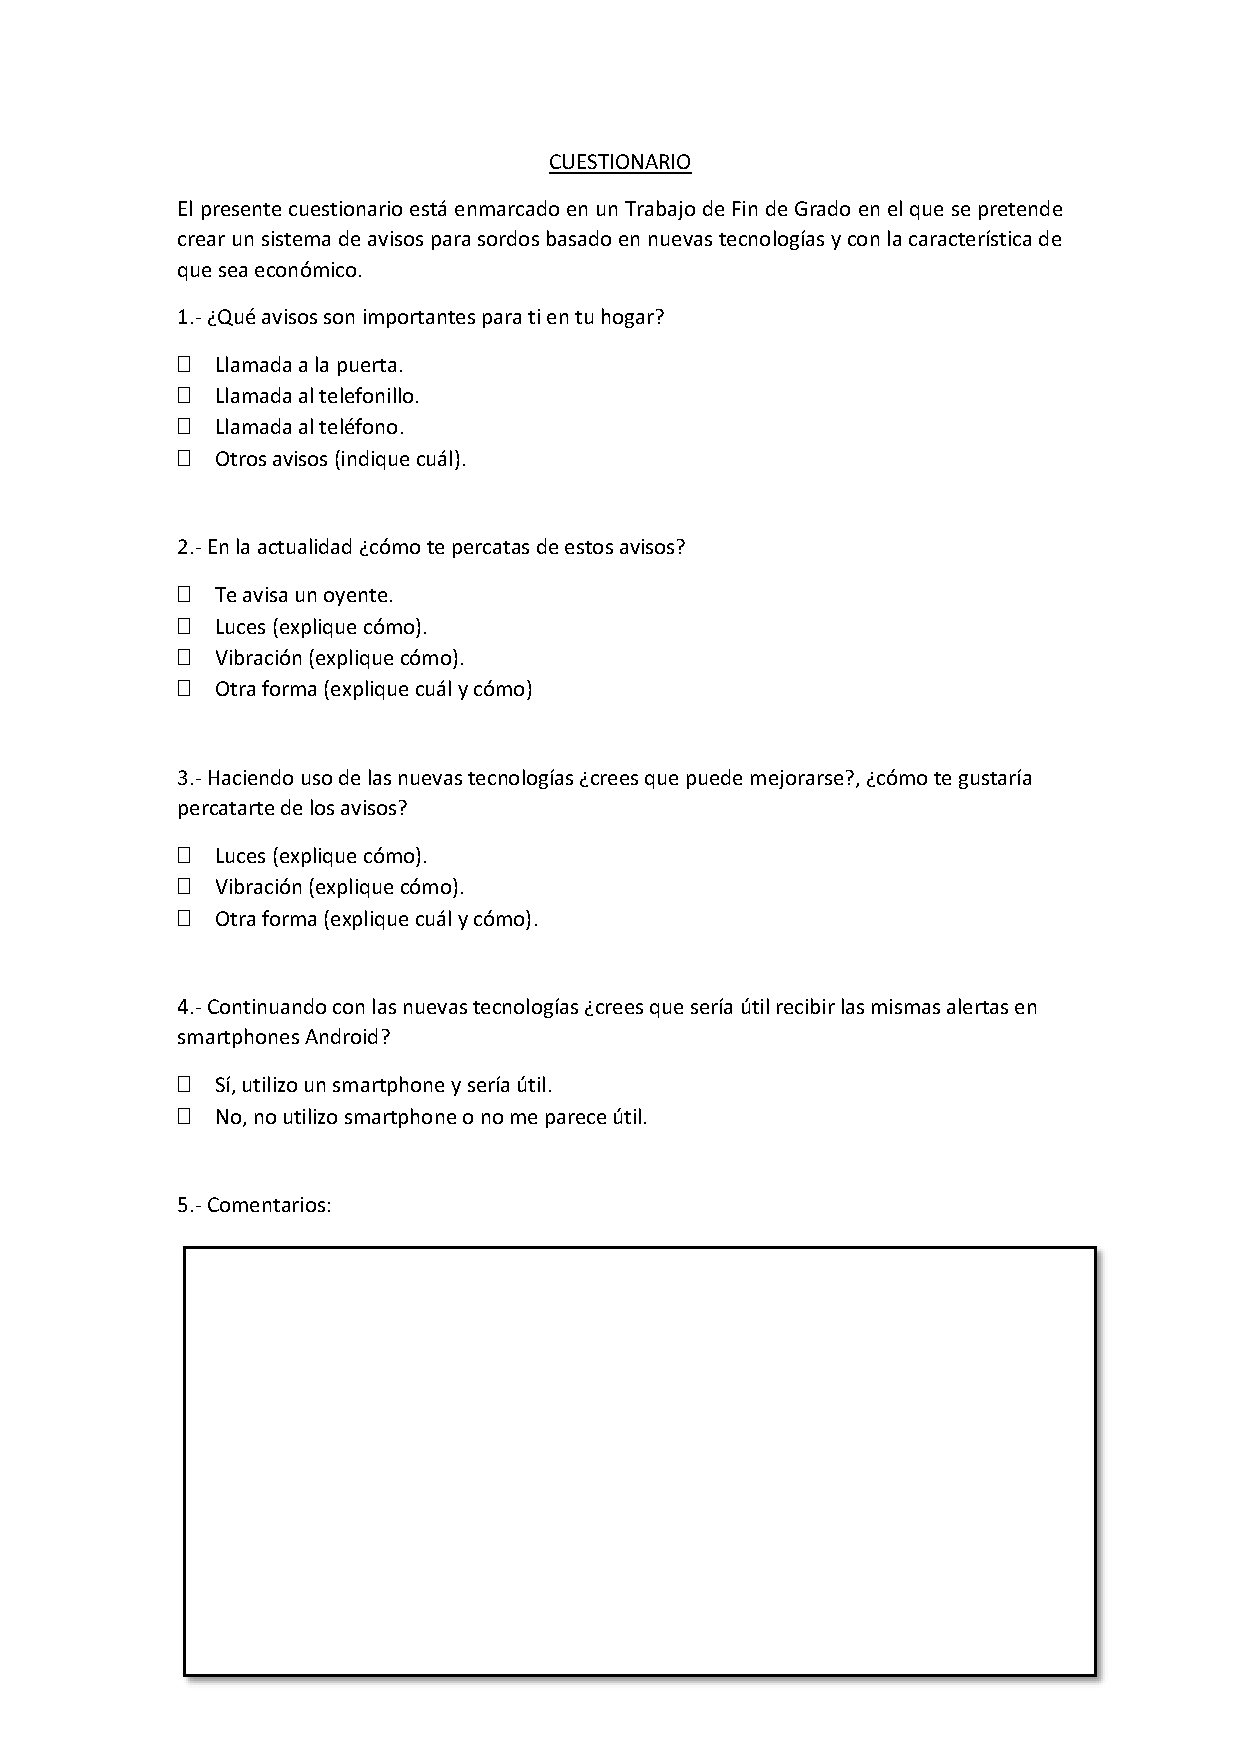
\includepdf[pages={1},scale=0.7,offset=-15 -45,pagecommand={\chapter{Documentación de Entrada}\section{Cuestionario realizado a personas con discapacidad auditiva}\label{sec:cuestionario}\pagestyle{fancytfg}}]{./contenido/content-anexos/cuestionario.pdf}

\clearpage
\chapter{Análisis y Diseño del Sistema}
\label{sec:analisisdiseno}

    \section{Análisis de requisitos específicos de sistema software}
    
    En este apartado se estudian los objetivos y requisitos específicos para cada sistema software utilizado, tanto el sistema desarrollado para el nodo central como la aplicación para smartphone, profundizando más allá de las Especificaciones del Sistema disponibles en el apartado~\ref{sec:especificaciones}.

        \subsection{Requisitos específicos de sistema central}
        
            \subsubsection{Objetivos específicos}
            
            \begin{table}[!ht]
                \centering
                \resizebox{\textwidth}{!}{%
               \begin{tabular}{|l|p{11cm}|}
                    \hline
                    \textbf{OBJ-01} & Utilizar puente Hue. \\ \hline
                    \textbf{Descripción} & El sistema deberá conectar con el puente Philips Hue empleado y poder realizar las operaciones necesarias. \\ \hline
                    \textbf{Importancia} & Alta. \\ \hline
                    \textbf{Estabilidad} & Alta. \\ \hline
                    \textbf{Comentarios} & Ninguno. \\ \hline
                \end{tabular}
                }
                \caption{Objetivo 1 del nodo central: Utilizar el puente Hue.}
               \label{sys_obj1}
            \end{table}
            
            \begin{table}[!ht]
                \centering
                \resizebox{\textwidth}{!}{%
               \begin{tabular}{|l|p{11cm}|}
                    \hline
                    \textbf{OBJ-02} & Detectar llamadas. \\ \hline
                    \textbf{Descripción} & El sistema deberá detectar las llamadas al timbre y al telefonillo. \\ \hline
                    \textbf{Importancia} & Alta. \\ \hline
                    \textbf{Estabilidad} & Alta. \\ \hline
                    \textbf{Comentarios} & Ninguno. \\ \hline
                \end{tabular}
                }
                \caption{Objetivo 2 del nodo central: Detectar llamadas.}
               \label{sys_obj2}
            \end{table}
            
            \begin{table}[!ht]
                \centering
                \resizebox{\textwidth}{!}{%
               \begin{tabular}{|l|p{11cm}|}
                    \hline
                    \textbf{OBJ-03} & Alertar mediante bombillas. \\ \hline
                    \textbf{Descripción} & El sistema deberá alertar al usuario mediante las bombillas, cambiando su estado. \\ \hline
                    \textbf{Importancia} & Alta. \\ \hline
                    \textbf{Estabilidad} & Alta. \\ \hline
                    \textbf{Comentarios} & Ninguno. \\ \hline
                \end{tabular}
                }
                \caption{Objetivo 3 del nodo central: Alertar mediante bombillas.}
               \label{sys_obj3}
            \end{table}
            
            \begin{table}[H]
                \centering
                \resizebox{\textwidth}{!}{%
               \begin{tabular}{|l|p{11cm}|}
                    \hline
                    \textbf{OBJ-04} & Alertar mediante smartphone. \\ \hline
                    \textbf{Descripción} & El sistema deberá alertar al usuario mediante el envío de alertas al smartphone. \\ \hline
                    \textbf{Importancia} & Alta. \\ \hline
                    \textbf{Estabilidad} & Alta. \\ \hline
                    \textbf{Comentarios} & Ninguno. \\ \hline
                \end{tabular}
                }
                \caption{Objetivo 4 del nodo central: Alertar mediante smartphone.}
               \label{sys_obj4}
            \end{table}
        
            \subsubsection{Requisitos funcionales específicos}
            
                \paragraph{Diagrama de Casos de Uso}\mbox{}\\
                
                \begin{figure}[!ht]
                  \centering
                    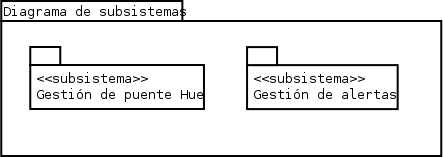
\includegraphics[width=0.6\textwidth]{subsistemas_casosuso_raspi.png}
                  \caption{Diagrama de subsistemas.}
                  \label{subsistemas_casosuso_raspi}
                \end{figure}
                
                \begin{figure}[H]
                  \centering
                    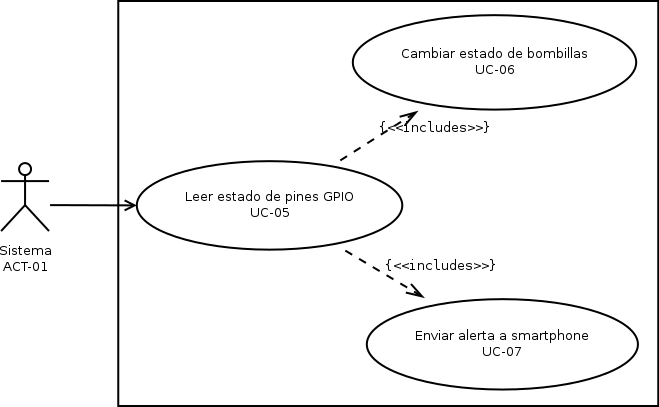
\includegraphics[width=0.7\textwidth]{casosuso_sub_alertas.png}
                  \caption{Diagrama de subsistema de gestión de alertas.}
                  \label{casosuso_sub_alertas}
                \end{figure}
                
                \begin{figure}[H]
                  \centering
                    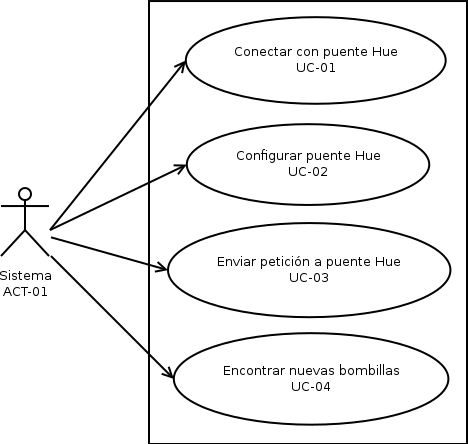
\includegraphics[width=0.6\textwidth]{casosuso_sub_hue.png}
                  \caption{Diagrama de subsistema de gestión de puente Hue.}
                  \label{casosuso_sub_hue}
                \end{figure}
                
                \paragraph{Definición de actores}\mbox{}\\

                \begin{table}[!ht]
                    \centering
                    \resizebox{\textwidth}{!}{%
                    \begin{tabular}{|l|p{11cm}|}
                        \hline
                        \textbf{ACT-01} & Sistema. \\ \hline
                        \textbf{Descripción} & Este actor representa al propio sistema nodo central, que tendrá funcionamiento automático y será el encargado de interactuar con los distintos elementos que lo conforman. \\ \hline
                    \end{tabular}
                    }
                    \caption{Actor 01: Sistema.}
                    \label{ACT01_sys}
                \end{table}
                
                
                \paragraph{Casos de Uso}\mbox{}\\
                
                    \subparagraph{Subsistema de gestión de puente Hue}\mbox{}\\
                    \clearpage
                
                    \begin{table}[!ht]
                        \centering
                        \resizebox{\textwidth}{!}{%
                        \begin{tabular}{|l|p{1cm}|p{9cm}|}
                            \hline
                            \textbf{UC-01} & \multicolumn{2}{|p{10cm}|}{Conectar con puente Hue.} \\ \hline
                            \textbf{Objetivos asociados} & \multicolumn{2}{|p{10cm}|}{\vspace{-2mm}\begin{itemize}[noitemsep,nosep]
                                                                \item OBJ-01 Utilizar el puente Hue.
                                                            \end{itemize}\vspace{-\baselineskip}\mbox{}} \\ \hline
                            \textbf{Descripción} & \multicolumn{2}{|p{10cm}|}{El sistema deberá comportarse tal como se describe en el siguiente caso de uso cuando se conecte con el puente Hue.}  \\ \hline
                            \textbf{Precondición} & \multicolumn{2}{|p{10cm}|}{El sistema no está conectado al puente Hue.} \\ \hline
                            \textbf{Secuencia normal} & \textbf{Paso} & \textbf{Acción} \\ \cline{2-3} & 1 & El sistema envía petición de conexión al puente Hue. \\ \cline{2-3} & 2 & Se establece la conexión. \\ \hline
                            \textbf{Postcondición} & \multicolumn{2}{|p{10cm}|}{El sistema queda conectado al puente Hue.} \\ \hline
                            \textbf{Excepciones} & \textbf{Paso} & \textbf{Acción} \\ \cline{2-3} & 2 & No se establece la conexión porque no se puede conectar con el puente Hue. A continuación este caso de uso queda sin efecto y el sistema debe reiniciarse. \\ \hline
                            \textbf{Rendimiento} & \textbf{Paso} & \textbf{Cota de tiempo} \\ \cline{2-3} & - & - \\ \hline
                            \textbf{Frecuencia} & \multicolumn{2}{|p{10cm}|}{1 vez.} \\ \hline
                            \textbf{Comentarios} & \multicolumn{2}{|p{10cm}|}{Ninguno} \\ \hline
                        \end{tabular}
                        }
                        \caption{Caso de Uso 01: Conectar con puente Hue.}
                        \label{UC01_sys}
                    \end{table}
                    
                    \begin{table}[H]
                        \centering
                        \resizebox{\textwidth}{!}{%
                        \begin{tabular}{|l|p{1cm}|p{9cm}|}
                            \hline
                            \textbf{UC-02} & \multicolumn{2}{|p{10cm}|}{Configurar puente Hue.} \\ \hline
                            \textbf{Objetivos asociados} & \multicolumn{2}{|p{10cm}|}{\vspace{-2mm}\begin{itemize}[noitemsep,nosep]
                                                                \item OBJ-01 Utilizar el puente Hue.
                                                            \end{itemize}\vspace{-\baselineskip}\mbox{}} \\ \hline
                            \textbf{Descripción} & \multicolumn{2}{|p{10cm}|}{El sistema deberá comportarse tal como se describe en el siguiente caso de uso cuando se realicen operaciones de configuración del puente Hue.}  \\ \hline
                            \textbf{Precondición} & \multicolumn{2}{|p{10cm}|}{El sistema está conectado al puente Hue.} \\ \hline
                            \textbf{Secuencia normal} & \textbf{Paso} & \textbf{Acción} \\ \cline{2-3} & 1 & El sistema envía configuración al puente Hue. \\ \cline{2-3} & 2 & El puente Hue devuelve información relacionada con la configuración. \\ \cline{2-3} & 3 & Se ha realizado la configuración. \\ \hline
                            \textbf{Postcondición} & \multicolumn{2}{|p{10cm}|}{El sistema queda configurado de acuerdo a los parámetros dados.} \\ \hline
                            \textbf{Excepciones} & \textbf{Paso} & \textbf{Acción} \\ \cline{2-3} & 3 & Hay errores en la configuración enviada y el puente Hue no se configura de acuerdo a esos parámetros. A continuación este caso de uso queda sin efecto y el sistema sigue su funcionamiento.\\ \hline
                            \textbf{Rendimiento} & \textbf{Paso} & \textbf{Cota de tiempo} \\ \cline{2-3} & - & - \\ \hline
                            \textbf{Frecuencia} & \multicolumn{2}{|p{10cm}|}{PD} \\ \hline
                            \textbf{Comentarios} & \multicolumn{2}{|p{10cm}|}{Ninguno} \\ \hline
                        \end{tabular}
                        }
                        \caption{Caso de Uso 02: Configurar puente Hue.}
                        \label{UC02_sys}
                    \end{table}
                    
                    \begin{table}[H]
                        \centering
                        \resizebox{\textwidth}{!}{%
                        \begin{tabular}{|l|p{1cm}|p{9cm}|}
                            \hline
                            \textbf{UC-03} & \multicolumn{2}{|p{10cm}|}{Enviar petición a puente Hue.} \\ \hline
                            \textbf{Objetivos asociados} & \multicolumn{2}{|p{10cm}|}{\vspace{-2mm}\begin{itemize}[noitemsep,nosep]
                                                                \item OBJ-01 Utilizar el puente Hue.
                                                            \end{itemize}\vspace{-\baselineskip}\mbox{}} \\ \hline
                            \textbf{Descripción} & \multicolumn{2}{|p{10cm}|}{El sistema deberá comportarse tal como se describe en el siguiente caso de uso cuando se realice cualquier operación para utilizar el puente Hue.}  \\ \hline
                            \textbf{Precondición} & \multicolumn{2}{|p{10cm}|}{El sistema está conectado al puente Hue.} \\ \hline
                            \textbf{Secuencia normal} & \textbf{Paso} & \textbf{Acción} \\ \cline{2-3} & 1 & El sistema envía datos al puente Hue. \\ \cline{2-3} & 2 & El puente Hue devuelve información relacionada con la petición realizada. \\ \hline
                            \textbf{Postcondición} & \multicolumn{2}{|p{10cm}|}{El sistema recibe información de la petición y actúa en consecuencia.} \\ \hline
                            \textbf{Excepciones} & \multicolumn{2}{|p{10cm}|}{Ninguna.} \\ \hline
                            \textbf{Rendimiento} & \textbf{Paso} & \textbf{Cota de tiempo} \\ \cline{2-3} & - & - \\ \hline
                            \textbf{Frecuencia} & \multicolumn{2}{|p{10cm}|}{PD} \\ \hline
                            \textbf{Comentarios} & \multicolumn{2}{|p{10cm}|}{Ninguno} \\ \hline
                        \end{tabular}
                        }
                        \caption{Caso de Uso 03: Enviar petición a puente Hue.}
                        \label{UC03_sys}
                    \end{table}
                    
                    \vspace{-0.5cm}
                    \begin{table}[H]
                        \centering
                        \resizebox{\textwidth}{!}{%
                        \begin{tabular}{|l|p{1cm}|p{9cm}|}
                            \hline
                            \textbf{UC-04} & \multicolumn{2}{|p{10cm}|}{Encontrar nuevas bombillas.} \\ \hline
                            \textbf{Objetivos asociados} & \multicolumn{2}{|p{10cm}|}{\vspace{-2mm}\begin{itemize}[noitemsep,nosep]
                                                                \item OBJ-01 Utilizar el puente Hue.
                                                            \end{itemize}\vspace{-\baselineskip}\mbox{}} \\ \hline
                            \textbf{Descripción} & \multicolumn{2}{|p{10cm}|}{El sistema deberá comportarse tal como se describe en el siguiente caso de uso cuando busque nuevas bombillas en el entorno para asociarlas.}  \\ \hline
                            \textbf{Precondición} & \multicolumn{2}{|p{10cm}|}{El sistema está conectado al puente Hue.} \\ \hline
                            \textbf{Secuencia normal} & \textbf{Paso} & \textbf{Acción} \\ \cline{2-3} & 1 & El sistema envía una petición al puente Hue para obtener información sobre nuevas bombillas. \\ \cline{2-3} & 2 & El puente Hue devuelve información sobre nuevas bombillas instaladas. \\ \cline{2-3} & 3 & El sistema asocia las nuevas bombillas instaladas. \\ \hline
                            \textbf{Postcondición} & \multicolumn{2}{|p{10cm}|}{Las nuevas bombillas instaladas quedan asociadas al sistema.} \\ \hline
                            \textbf{Excepciones} & \textbf{Paso} & \textbf{Acción} \\ \cline{2-3} & 3 & No hay nuevas bombillas instaladas. A continuación este caso de uso queda sin efecto y el sistema sigue su funcionamiento. \\ \hline
                            \textbf{Rendimiento} & \textbf{Paso} & \textbf{Cota de tiempo} \\ \cline{2-3} & - & - \\ \hline
                            \textbf{Frecuencia} & \multicolumn{2}{|p{10cm}|}{PD} \\ \hline
                            \textbf{Comentarios} & \multicolumn{2}{|p{10cm}|}{Ninguno} \\ \hline
                        \end{tabular}
                        }
                        \caption{Caso de Uso 04: Encontrar nuevas bombillas.}
                        \label{UC04_sys}
                    \end{table}
                    
                    \subparagraph{Subsistema de gestión de alertas}\mbox{}\\
                
                    \begin{table}[H]
                        \centering
                        \resizebox{\textwidth}{!}{%
                        \begin{tabular}{|l|p{1cm}|p{9cm}|}
                            \hline
                            \textbf{UC-05} & \multicolumn{2}{|p{10cm}|}{Leer estado de pines GPIO.} \\ \hline
                            \textbf{Objetivos asociados} & \multicolumn{2}{|p{10cm}|}{\vspace{-2mm}\begin{itemize}[noitemsep,nosep]
                                                                \item OBJ-02 Detectar llamadas.
                                                            \end{itemize}\vspace{-\baselineskip}\mbox{}} \\ \hline
                            \textbf{Descripción} & \multicolumn{2}{|p{10cm}|}{El sistema deberá comportarse tal como se describe en el siguiente caso de uso cuando se reciba una señal a través de los pines GPIO.}  \\ \hline
                            \textbf{Precondición} & \multicolumn{2}{|p{10cm}|}{El sistema recibe una señal eléctrica TTL a través de GPIO.} \\ \hline
                            \textbf{Secuencia normal} & \textbf{Paso} & \textbf{Acción} \\ \cline{2-3} & 1 & El sistema filtra la señal a través de GPIO. \\ \cline{2-3} & 2 & El sistema discrimina si es una señal del telefonillo o del timbre. \\ \hline
                            \textbf{Postcondición} & \multicolumn{2}{|p{10cm}|}{El sistema realiza las acciones determinadas en los casos de uso UC-06 y UC-07.} \\ \hline
                            \textbf{Excepciones} & \multicolumn{2}{|p{10cm}|}{Ninguna} \\ \hline
                            \textbf{Rendimiento} & \textbf{Paso} & \textbf{Cota de tiempo} \\ \cline{2-3} & - & - \\ \hline
                            \textbf{Frecuencia} & \multicolumn{2}{|p{10cm}|}{PD} \\ \hline
                            \textbf{Comentarios} & \multicolumn{2}{|p{10cm}|}{Ninguno} \\ \hline
                        \end{tabular}
                        }
                        \caption{Caso de Uso 05: Leer estado de pines GPIO.}
                        \label{UC05_sys}
                    \end{table}
                    
                    \begin{table}[H]
                        \centering
                        \resizebox{\textwidth}{!}{%
                        \begin{tabular}{|l|p{1cm}|p{9cm}|}
                            \hline
                            \textbf{UC-06} & \multicolumn{2}{|p{10cm}|}{Cambiar estado de bombillas.} \\ \hline
                            \textbf{Objetivos asociados} & \multicolumn{2}{|p{10cm}|}{\vspace{-2mm}\begin{itemize}[noitemsep,nosep]
                                                                \item OBJ-03 Alertar mediante bombillas.
                                                            \end{itemize}\vspace{-\baselineskip}\mbox{}} \\ \hline
                            \textbf{Descripción} & \multicolumn{2}{|p{10cm}|}{El sistema deberá comportarse tal como se describe en el siguiente caso de uso cuando termine el caso de uso UC-05.}  \\ \hline
                            \textbf{Precondición} & \multicolumn{2}{|p{10cm}|}{El sistema está conectado al puente Hue y acaba de terminar el caso de uso UC-05.} \\ \hline
                            \textbf{Secuencia normal} & \textbf{Paso} & \textbf{Acción} \\ \cline{2-3} & 1 & El sistema almacena el antiguo estado de las bombillas conectadas. \\ \cline{2-3} & 2 & El sistema envía petición de cambio de estado de las bombillas al puente Hue, de acuerdo a la salida del caso de uso UC-05. \\ \cline{2-3} & 3 & El sistema vuelve a enviar una petición de cambio de estado al puente Hue para revertir el cambio, estableciendo ahora el antiguo estado. \\ \hline
                            \textbf{Postcondición} & \multicolumn{2}{|p{10cm}|}{El sistema vuelve a quedar en estado de espera de alertas.} \\ \hline
                            \textbf{Excepciones} & \multicolumn{2}{|p{10cm}|}{Ninguna} \\ \hline
                            \textbf{Rendimiento} & \textbf{Paso} & \textbf{Cota de tiempo} \\ \cline{2-3} & - & - \\ \hline
                            \textbf{Frecuencia} & \multicolumn{2}{|p{10cm}|}{PD} \\ \hline
                            \textbf{Comentarios} & \multicolumn{2}{|p{10cm}|}{Ninguno} \\ \hline
                        \end{tabular}
                        }
                        \caption{Caso de Uso 06: Cambiar estado de bombillas.}
                        \label{UC06_sys}
                    \end{table}
                    
                    \begin{table}[H]
                        \centering
                        \resizebox{\textwidth}{!}{%
                        \begin{tabular}{|l|p{1cm}|p{9cm}|}
                            \hline
                            \textbf{UC-07} & \multicolumn{2}{|p{10cm}|}{Enviar alerta a smartphone.} \\ \hline
                            \textbf{Objetivos asociados} & \multicolumn{2}{|p{10cm}|}{\vspace{-2mm}\begin{itemize}[noitemsep,nosep]
                                                                \item OBJ-04 Alertar mediante smartphone.
                                                            \end{itemize}\vspace{-\baselineskip}\mbox{}} \\ \hline
                            \textbf{Descripción} & \multicolumn{2}{|p{10cm}|}{El sistema deberá comportarse tal como se describe en el siguiente caso de uso cuando termine el caso de uso UC-05.}  \\ \hline
                            \textbf{Precondición} & \multicolumn{2}{|p{10cm}|}{El sistema acaba de terminar el caso de uso UC-05.} \\ \hline
                            \textbf{Secuencia normal} & \textbf{Paso} & \textbf{Acción} \\ \cline{2-3} & 1 & El sistema espera a solicitud de alerta por parte del smartphone. \\ \cline{2-3} & 2 & El sistema envía la alerta al smartphone a modo de texto, de acuerdo a la salida del caso de uso UC-05. \\ \hline
                            \textbf{Postcondición} & \multicolumn{2}{|p{10cm}|}{El sistema vuelve a quedar en estado de espera de alertas.} \\ \hline
                            \textbf{Excepciones} & \multicolumn{2}{|p{10cm}|}{Ninguna} \\ \hline
                            \textbf{Rendimiento} & \textbf{Paso} & \textbf{Cota de tiempo} \\ \cline{2-3} & - & - \\ \hline
                            \textbf{Frecuencia} & \multicolumn{2}{|p{10cm}|}{PD} \\ \hline
                            \textbf{Comentarios} & \multicolumn{2}{|p{10cm}|}{Ninguno} \\ \hline
                        \end{tabular}
                        }
                        \caption{Caso de Uso 07: Enviar alerta a smartphone.}
                        \label{UC07_sys}
                    \end{table}

        \subsection{Requisitos específicos de aplicación para smartphone}
        
            \subsubsection{Objetivos específicos}
            
            \begin{table}[!ht]
                \centering
                \resizebox{\textwidth}{!}{%
               \begin{tabular}{|l|p{11cm}|}
                    \hline
                    \textbf{OBJ-01} & Conectar con nodo central. \\ \hline
                    \textbf{Descripción} & El sistema deberá permitir la conexión con el nodo central y la configuración de esta conexión. \\ \hline
                    \textbf{Importancia} & Alta. \\ \hline
                    \textbf{Estabilidad} & Alta. \\ \hline
                    \textbf{Comentarios} & Ninguno. \\ \hline
                \end{tabular}
                }
                \caption{Objetivo 1 de la aplicación para smartphone: Conectar con nodo central.}
               \label{android_obj1}
            \end{table}
            
            \begin{table}[!ht]
                \centering
                \resizebox{\textwidth}{!}{%
               \begin{tabular}{|l|p{11cm}|}
                    \hline
                    \textbf{OBJ-02} & Mostrar alerta a usuario. \\ \hline
                    \textbf{Descripción} & El sistema deberá mostrar las alertas recibidas en modo texto al usuario. \\ \hline
                    \textbf{Importancia} & Alta. \\ \hline
                    \textbf{Estabilidad} & Alta. \\ \hline
                    \textbf{Comentarios} & Ninguno. \\ \hline
                \end{tabular}
                }
                \caption{Objetivo 2 de la aplicación para smartphone: Mostrar alerta a usuario.}
               \label{android_obj2}
            \end{table}
            
            \begin{table}[H]
                \centering
                \resizebox{\textwidth}{!}{%
               \begin{tabular}{|l|p{11cm}|}
                    \hline
                    \textbf{OBJ-03} & Gestionar alertas. \\ \hline
                    \textbf{Descripción} & El sistema deberá permitir la gestión de las alertas por parte del usuario. \\ \hline
                    \textbf{Importancia} & Alta. \\ \hline
                    \textbf{Estabilidad} & Alta. \\ \hline
                    \textbf{Comentarios} & Ninguno. \\ \hline
                \end{tabular}
                }
                \caption{Objetivo 3 de la aplicación para smartphone: Gestionar alertas.}
               \label{android_obj3}
            \end{table}
        
            \subsubsection{Requisitos funcionales específicos}
            
                \paragraph{Diagrama de Casos de Uso}\mbox{}\\
                
                \begin{figure}[!ht]
                  \centering
                    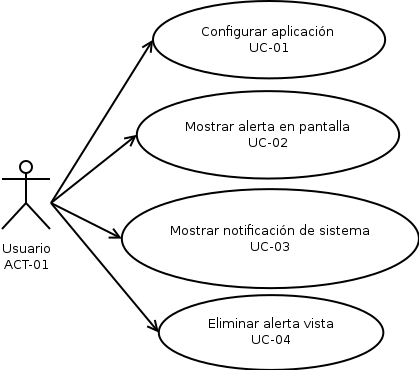
\includegraphics[width=0.6\textwidth]{casosuso_android.png}
                  \caption{Diagrama de casos de uso de aplicación para smartphone.}
                  \label{casosuso_android}
                \end{figure}
                
                \paragraph{Definición de actores}\mbox{}\\

                \begin{table}[!ht]
                    \centering
                    \resizebox{\textwidth}{!}{%
                    \begin{tabular}{|l|p{11cm}|}
                        \hline
                        \textbf{ACT-01} & Usuario. \\ \hline
                        \textbf{Descripción} & Este actor representa al usuario de la aplicación para smartphone. \\ \hline
                    \end{tabular}
                    }
                    \caption{Actor 01: Usuario.}
                    \label{ACT01_android}
                \end{table}
                
                \paragraph{Casos de Uso}\mbox{}\\
                
                \begin{table}[!ht]
                    \centering
                    \resizebox{\textwidth}{!}{%
                    \begin{tabular}{|l|p{1cm}|p{9cm}|}
                        \hline
                        \textbf{UC-01} & \multicolumn{2}{|p{10cm}|}{Configurar aplicación.} \\ \hline
                        \textbf{Objetivos asociados} & \multicolumn{2}{|p{10cm}|}{\vspace{-2mm}\begin{itemize}[noitemsep,nosep]
                                                            \item OBJ-01 Conectar con nodo central.
                                                        \end{itemize}\vspace{-\baselineskip}\mbox{}} \\ \hline
                        \textbf{Descripción} & \multicolumn{2}{|p{10cm}|}{El sistema deberá comportarse tal como se describe en el siguiente caso de uso cuando el usuario configure la aplicación.}  \\ \hline
                        \textbf{Precondición} & \multicolumn{2}{|p{10cm}|}{El usuario ha accedido a la configuración del sistema.} \\ \hline
                        \textbf{Secuencia normal} & \textbf{Paso} & \textbf{Acción} \\ \cline{2-3} & 1 & El sistema muestra un menú de configuración donde introducir la dirección del nodo central. \\ \cline{2-3} & 2 & Se comprueba la dirección del nodo central. \\ \cline{2-3} & 3 & La dirección es correcta y el sistema conecta con el nodo central. \\ \hline
                        \textbf{Postcondición} & \multicolumn{2}{|p{10cm}|}{El sistema queda conectado al nodo central.} \\ \hline
                        \textbf{Excepciones} & \textbf{Paso} & \textbf{Acción} \\ \cline{2-3} & 3 & La dirección proporcionada por el usuario es incorrecta y el sistema no conecta con el nodo central. A continuación este caso de uso se reinicia. \\ \hline
                        \textbf{Rendimiento} & \textbf{Paso} & \textbf{Cota de tiempo} \\ \cline{2-3} & - & - \\ \hline
                        \textbf{Frecuencia} & \multicolumn{2}{|p{10cm}|}{PD} \\ \hline
                        \textbf{Comentarios} & \multicolumn{2}{|p{10cm}|}{Ninguno} \\ \hline
                    \end{tabular}
                    }
                    \caption{Caso de Uso 01: Configurar aplicación.}
                    \label{UC01_app}
                \end{table}
                
                \begin{table}[!ht]
                    \centering
                    \resizebox{\textwidth}{!}{%
                    \begin{tabular}{|l|p{1cm}|p{9cm}|}
                        \hline
                        \textbf{UC-02} & \multicolumn{2}{|p{10cm}|}{Mostrar alerta en pantalla.} \\ \hline
                        \textbf{Objetivos asociados} & \multicolumn{2}{|p{10cm}|}{\vspace{-2mm}\begin{itemize}[noitemsep,nosep]
                                                            \item OBJ-02 Mostrar alerta a usuario.
                                                        \end{itemize}\vspace{-\baselineskip}\mbox{}} \\ \hline
                        \textbf{Descripción} & \multicolumn{2}{|p{10cm}|}{El sistema deberá comportarse tal como se describe en el siguiente caso de uso cuando se recibe una alerta del nodo central.}  \\ \hline
                        \textbf{Precondición} & \multicolumn{2}{|p{10cm}|}{El usuario ha accedido a la pantalla principal de la aplicación y la aplicación se encuentra en primer plano.} \\ \hline
                        \textbf{Secuencia normal} & \textbf{Paso} & \textbf{Acción} \\ \cline{2-3} & 1 & El sistema recibe una alerta del nodo central. \\ \cline{2-3} & 2 & Se almacena la alerta temporalmente y se muestra por pantalla. \\ \cline{2-3} & 3 & El usuario ve la alerta, pudiendo pasar al caso de uso UC-04. \\ \hline
                        \textbf{Postcondición} & \multicolumn{2}{|p{10cm}|}{El sistema queda a la espera de más alertas.} \\ \hline
                        \textbf{Excepciones} & \multicolumn{2}{|p{10cm}|}{Ninguna} \\ \hline
                        \textbf{Rendimiento} & \textbf{Paso} & \textbf{Cota de tiempo} \\ \cline{2-3} & - & - \\ \hline
                        \textbf{Frecuencia} & \multicolumn{2}{|p{10cm}|}{PD} \\ \hline
                        \textbf{Comentarios} & \multicolumn{2}{|p{10cm}|}{Ninguno} \\ \hline
                    \end{tabular}
                    }
                    \caption{Caso de Uso 02: Mostrar alerta en pantalla.}
                    \label{UC02_app}
                \end{table}
                
                \begin{table}[!ht]
                    \centering
                    \resizebox{\textwidth}{!}{%
                    \begin{tabular}{|l|p{1cm}|p{9cm}|}
                        \hline
                        \textbf{UC-03} & \multicolumn{2}{|p{10cm}|}{Mostrar notificación en sistema.} \\ \hline
                        \textbf{Objetivos asociados} & \multicolumn{2}{|p{10cm}|}{\vspace{-2mm}\begin{itemize}[noitemsep,nosep]
                                                            \item OBJ-02 Mostrar alerta a usuario.
                                                        \end{itemize}\vspace{-\baselineskip}\mbox{}} \\ \hline
                        \textbf{Descripción} & \multicolumn{2}{|p{10cm}|}{El sistema deberá comportarse tal como se describe en el siguiente caso de uso cuando se recibe una alerta del nodo central.}  \\ \hline
                        \textbf{Precondición} & \multicolumn{2}{|p{10cm}|}{El usuario tiene la aplicación funcionando en segundo plano.} \\ \hline
                        \textbf{Secuencia normal} & \textbf{Paso} & \textbf{Acción} \\ \cline{2-3} & 1 & El sistema recibe una alerta del nodo central. \\ \cline{2-3} & 2 & Se almacena la alerta temporalmente y se envía una notificación al sistema. \\ \cline{2-3} & 3 & El usuario ve la notificación, pudiendo pasar al caso de uso UC-04. \\ \hline
                        \textbf{Postcondición} & \multicolumn{2}{|p{10cm}|}{El sistema queda a la espera de más alertas.} \\ \hline
                        \textbf{Excepciones} & \multicolumn{2}{|p{10cm}|}{Ninguna} \\ \hline
                        \textbf{Rendimiento} & \textbf{Paso} & \textbf{Cota de tiempo} \\ \cline{2-3} & - & - \\ \hline
                        \textbf{Frecuencia} & \multicolumn{2}{|p{10cm}|}{PD} \\ \hline
                        \textbf{Comentarios} & \multicolumn{2}{|p{10cm}|}{Ninguno} \\ \hline
                    \end{tabular}
                    }
                    \caption{Caso de Uso 03: Mostrar notificación en sistema.}
                    \label{UC03_app}
                \end{table}
                
                \begin{table}[H]
                    \centering
                    \resizebox{\textwidth}{!}{%
                    \begin{tabular}{|l|p{1cm}|p{9cm}|}
                        \hline
                        \textbf{UC-04} & \multicolumn{2}{|p{10cm}|}{Eliminar alerta vista.} \\ \hline
                        \textbf{Objetivos asociados} & \multicolumn{2}{|p{10cm}|}{\vspace{-2mm}\begin{itemize}[noitemsep,nosep]
                                                            \item OBJ-03 Gestionar alertas.
                                                        \end{itemize}\vspace{-\baselineskip}\mbox{}} \\ \hline
                        \textbf{Descripción} & \multicolumn{2}{|p{10cm}|}{El sistema deberá comportarse tal como se describe en el siguiente caso de uso cuando el usuario pulsa sobre una alerta.}  \\ \hline
                        \textbf{Precondición} & \multicolumn{2}{|p{10cm}|}{El usuario pulsa sobre una alerta.} \\ \hline
                        \textbf{Secuencia normal} & \textbf{Paso} & \textbf{Acción} \\ \cline{2-3} & 1 & El sistema comprueba la alerta sobre la que se pulsa. \\ \cline{2-3} & 2 & El sistema muestra un diálogo para que el usuario acepte eliminar la alerta. \\ \cline{2-3} & 3 & El usuario acepta eliminar la alerta. \\ \cline{2-3} & 4 & El sistema elimina la alerta de la lista temporal. \\ \hline
                        \textbf{Postcondición} & \multicolumn{2}{|p{10cm}|}{El sistema queda a la espera de más alertas.} \\ \hline
                        \textbf{Excepciones} & \textbf{Paso} & \textbf{Acción} \\ \cline{2-3} & 3 & El usuario no acepta eliminar la alerta. A continuación este caso de uso queda sin efecto y el sistema sigue su funcionamiento. \\ \hline
                        \textbf{Rendimiento} & \textbf{Paso} & \textbf{Cota de tiempo} \\ \cline{2-3} & - & - \\ \hline
                        \textbf{Frecuencia} & \multicolumn{2}{|p{10cm}|}{PD} \\ \hline
                        \textbf{Comentarios} & \multicolumn{2}{|p{10cm}|}{Ninguno} \\ \hline
                    \end{tabular}
                    }
                    \caption{Caso de Uso 04: Eliminar alerta vista.}
                    \label{UC04_app}
                \end{table}
            

    \section{Diseño software del sistema}
    
    De acuerdo al análisis realizado en el apartado anterior, el diseño de software para el sistema software del nodo central y el diseño de software para la aplicación para smartphone queda definido en las figuras~\ref{diagrama_clases_py} y~\ref{diagrama_clases_android}, respectivamente.
    
    \begin{figure}[!ht]
      \centering
        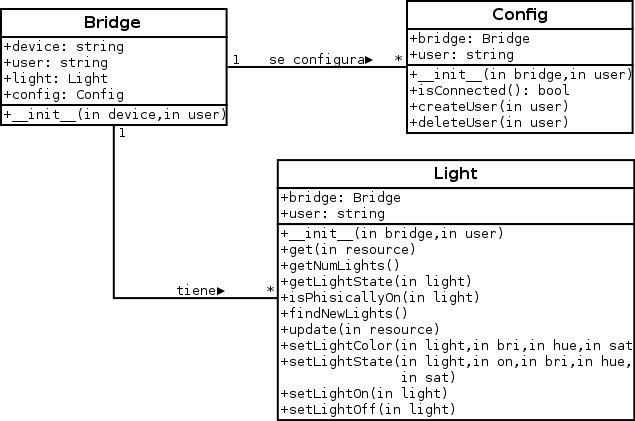
\includegraphics[width=0.7\textwidth]{diagrama_clases_py.png}
      \caption{Diagrama de diseño del sistema software del nodo central.}
      \label{diagrama_clases_py}
    \end{figure}
    
    \begin{figure}[H]
      \centering
        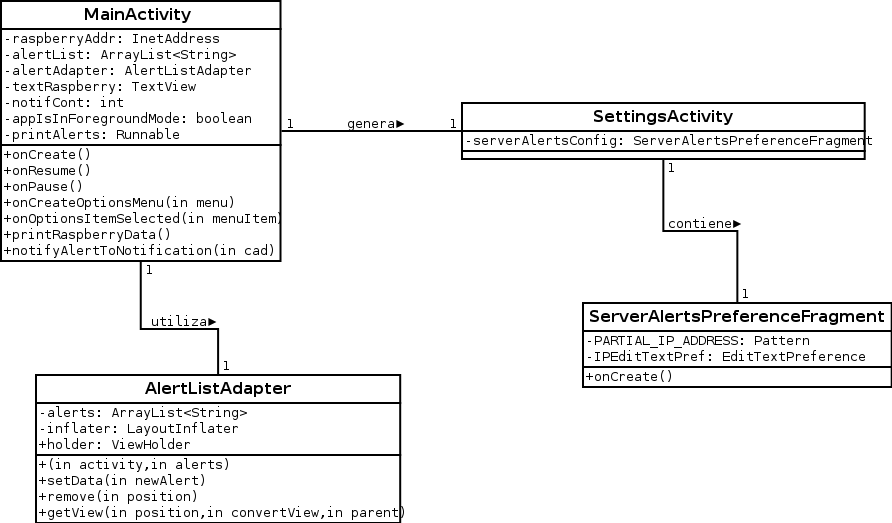
\includegraphics[width=0.9\textwidth]{diagrama_clases_android.png}
      \caption{Diagrama de diseño de la aplicación para smartphone.}
      \label{diagrama_clases_android}
    \end{figure}

    \section{Diseño de prototipo de aplicación para smartphone}
    \label{sec:disenoapp}

    El diseño del prototipo de la aplicación se compone de una pantalla principal con la lista de alertas y un botón para menú de configuración (figuras~\ref{disenoapp_1} y~\ref{disenoapp_2}), un sistema de borrado de alertas mediante ventanas emergentes (figura~\ref{disenoapp_3}), y un menú de configuración (figura~\ref{disenoapp_4}) en el que se pueda introducir la dirección del servidor de alertas, el nodo central del sistema. \\

    \begin{figure}[!ht]
      \centering
      {%
        \setlength{\fboxsep}{0pt}%
        \setlength{\fboxrule}{1pt}%
        \fbox{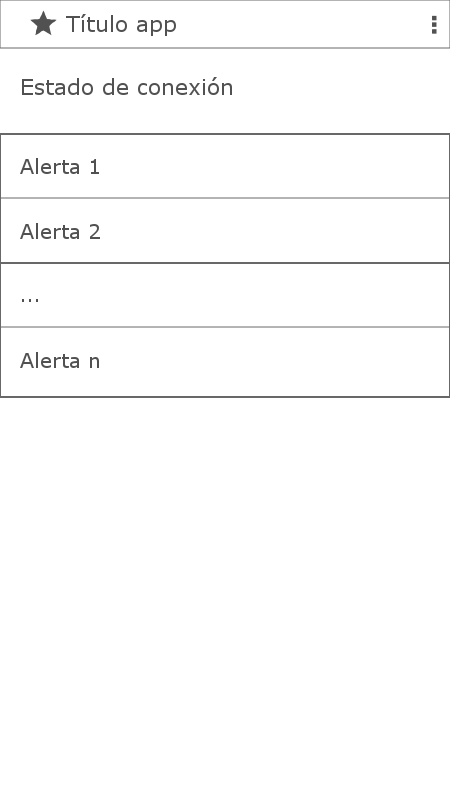
\includegraphics[width=0.3\textwidth]{disenoapp_1.png}}
      }%
      \caption{Prototipo de la pantalla principal de la aplicación para smartphones.}
      \label{disenoapp_1}
    \end{figure}

    \begin{figure}[!ht]
      \centering
      {%
        \setlength{\fboxsep}{0pt}%
        \setlength{\fboxrule}{1pt}%
        \fbox{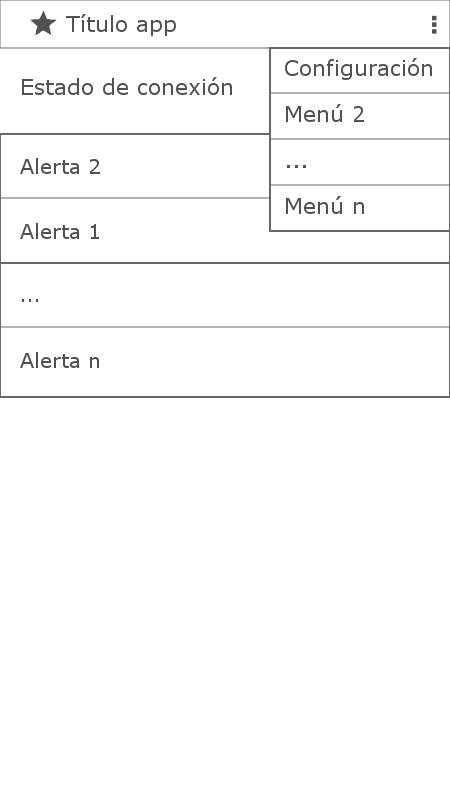
\includegraphics[width=0.3\textwidth]{disenoapp_3.png}}
      }%
      \caption{Prototipo del menú desplegable.}
      \label{disenoapp_2}
    \end{figure}

    \begin{figure}[!ht]
      \centering
      {%
        \setlength{\fboxsep}{0pt}%
        \setlength{\fboxrule}{1pt}%
        \fbox{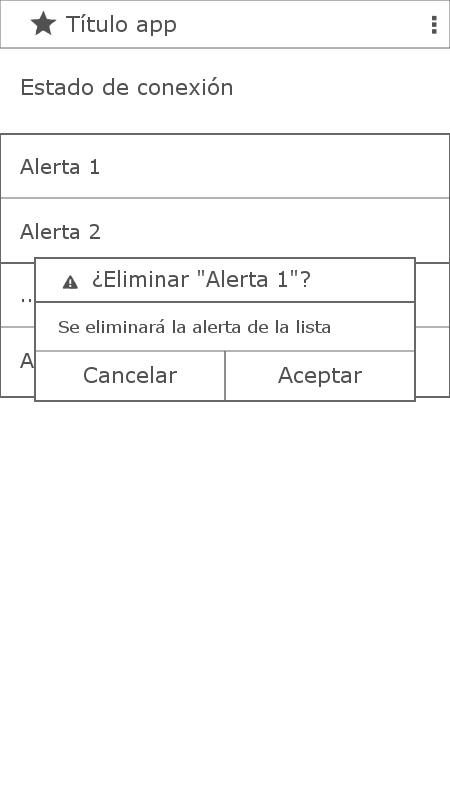
\includegraphics[width=0.3\textwidth]{disenoapp_2.png}}
      }%
      \caption{Prototipo de ventana emergente para eliminar alertas.}
      \label{disenoapp_3}
    \end{figure}

    \clearpage
    \begin{figure}[!ht]
      \centering
      {%
        \setlength{\fboxsep}{0pt}%
        \setlength{\fboxrule}{1pt}%
        \fbox{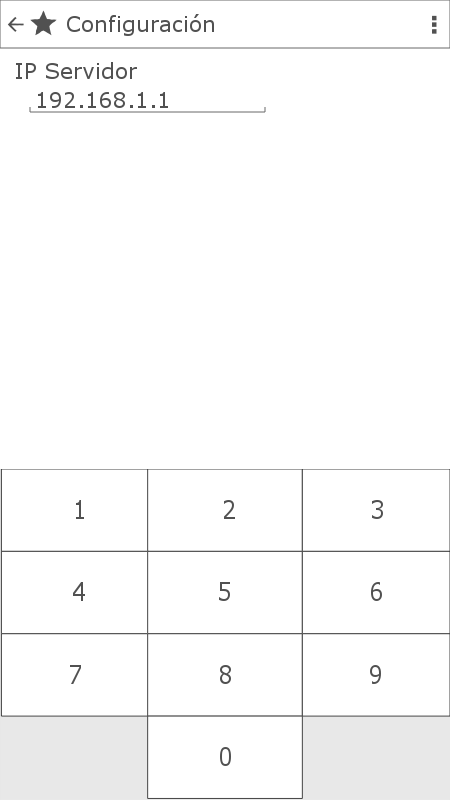
\includegraphics[width=0.3\textwidth]{disenoapp_4.png}}
      }%
      \caption{Prototipo de menú de configuración.}
      \label{disenoapp_4}
    \end{figure}
    
\clearpage
\chapter{Plan de Pruebas}
\label{pruebas}
    
    \section{Trazabilidad de Casos de Prueba - Requisitos}
    
    En este apartado se expone la tabla~\ref{trazabilidad} que muestra la trazabilidad entre Casos de Prueba y Requisitos Funcionales (Casos de Uso), tanto requisitos generales, como requisitos específicos de cada subsistema software, es decir, se expone que se satisfacen los requisitos para cada Caso de Prueba.
        
        \begin{table}[H] 
            \begin{adjustwidth}{-.5in}{-.5in}
            \centering
            \resizebox{1.06\textwidth}{!}{%
            \begin{tabular}{||c||c|c|c|c||c|c|c|c|c|c|c||c|c|c|c||}
                \hline
                \multirow{2}{*}{} & \multicolumn{4}{c||}{Requisitos Generales} & \multicolumn{7}{c||}{Requisitos Específicos Sistema Central} & \multicolumn{4}{c||}{\begin{tabular}[x]{@{}c@{}}Requisitos Específicos Aplicación\\para smartphone\end{tabular}} \\ \cline{2-16}
                & UC-01 & UC-02 & UC-03 & UC-04 & UC-01 & UC-02 & UC-03 & UC-04 & UC-05 & UC-06 & UC-07 & UC-01 & UC-02 & UC-03 & UC-04 \\ \hhline{#=#====#=======#====#}
            %%  CP-0X & 01& 02& 03& 04& 01& 02& 03& 04& 05& 06& 07& 01& 02& 03& 04  
                CP-01 &   &   & X &   & X & X & X &   & X & X &   &   &   &   &   \\ \hline
                CP-02 &   &   &   & X &   &   &   &   & X &   & X & X & X &   &   \\ \hline
                CP-03 &   &   & X &   & X & X & X & X & X & X &   &   &   &   &   \\ \hline
                CP-04 & X &   & X & X & X & X & X &   & X & X & X & X & X &   &   \\ \hline
                CP-05 &   & X & X & X & X & X & X &   & X & X & X & X & X &   &   \\ \hline
                CP-06 &   &   &   & X &   &   &   &   & X &   & X & X &   & X &   \\ \hline
                CP-07 &   &   &   & X &   &   &   &   & X &   & X & X & X & X & X \\ \hline
                CP-08 & X & X & X & X & X & X & X &   & X & X & X & X & X &   &   \\ \hline
                CP-09 & X & X & X &   & X & X & X & X & X & X &   &   &   &   &   \\ \hline
            \end{tabular}
            }
            \caption{Trazabilidad de Casos de Prueba - Requisitos (Casos de Uso)}
            \label{trazabilidad}
            \end{adjustwidth}
        \end{table}
    
    \section{Definición de los Casos de Prueba}
    
    \begin{table}[H]
        \centering
        \resizebox{0.8\textwidth}{!}{%
        \begin{tabular}{|p{10.5cm}|c|}
            \hline
            \textbf{Comprobar recepción de alertas en Raspberry Pi y Hue} & CP-01 \\ \hline
            \multicolumn{2}{|p{12.2cm}|}{\begin{tabular}[x]{@{}p{12.2cm}@{}}\textbf{Descripción:}\\Mediante este Caso de Prueba se pretende comprobar la recepción de las alertas visuales en las bombillas Philips Hue. \end{tabular}} \\ \hline
            \multicolumn{2}{|p{12.2cm}|}{\begin{tabular}[x]{@{}p{12.2cm}@{}}\textbf{Prerrequisitos:}\\El sistema está conectado y encendido. Hay al menos una bombilla Hue encendida. \end{tabular}} \\ \hline
            \multicolumn{2}{|p{12.2cm}|}{\begin{tabular}[x]{@{}p{12.2cm}@{}}\textbf{Pasos:}\\ \vspace{-2mm}\begin{itemize}[noitemsep,nosep]
                \item Se pulsa el interruptor del timbre o del telefonillo.
                \item Se espera a ver las alertas en las bombillas Hue.
            \end{itemize}\vspace{-\baselineskip}\mbox{} \end{tabular}} \\ \hline
            \multicolumn{2}{|p{12.2cm}|}{\begin{tabular}[x]{@{}p{12.2cm}@{}}\textbf{Resultado esperado:}\\ Las bombillas Hue conectadas y encendidas físicamente parpadean entre un color y el estado anterior, mostrando así la alerta. \end{tabular}} \\ \hline
            \multicolumn{2}{|p{12.2cm}|}{\begin{tabular}[x]{@{}p{12.2cm}@{}}\textbf{Resultado obtenido:}\\Las bombillas Hue conectadas parpadean entre un color y el estado anterior, mostrando así la alerta. El resultado es el esperado. \end{tabular}} \\ \hline
        \end{tabular}
        }
        \caption{CP-01: Comprobar recepción de alertas en Raspberry Pi y Hue}
        \label{CP_01}
    \end{table}
    
    \begin{table}[H]
        \centering
        \resizebox{0.8\textwidth}{!}{%
        \begin{tabular}{|p{10.5cm}|c|}
            \hline
            \textbf{Comprobar recepción de alertas en smartphone} & CP-02 \\ \hline
            \multicolumn{2}{|p{12.2cm}|}{\begin{tabular}[x]{@{}p{12.2cm}@{}}\textbf{Descripción:}\\Mediante este Caso de Prueba se pretende comprobar la recepción de las alertas en la aplicación para smartphone. \end{tabular}} \\ \hline
            \multicolumn{2}{|p{12.2cm}|}{\begin{tabular}[x]{@{}p{12.2cm}@{}}\textbf{Prerrequisitos:}\\El sistema está conectado y encendido. Un smartphone con la aplicación instalada está conectado al sistema. \end{tabular}} \\ \hline
            \multicolumn{2}{|p{12.2cm}|}{\begin{tabular}[x]{@{}p{12.2cm}@{}}\textbf{Pasos:}\\ \vspace{-2mm}\begin{itemize}[noitemsep,nosep]
                \item Se inicia la aplicación para smartphone.
                \item Se pulsa el interruptor del timbre o del telefonillo.
                \item Se espera a recibir la alerta en la aplicación para smartphone.
                \item Se muestra una alerta con la fecha y hora, así como el evento ocurrido.
            \end{itemize}\vspace{-\baselineskip}\mbox{} \end{tabular}} \\ \hline
            \multicolumn{2}{|p{12.2cm}|}{\begin{tabular}[x]{@{}p{12.2cm}@{}}\textbf{Resultado esperado:}\\ Se recibe una alerta en la aplicación del smartphone que se muestra en la pantalla principal, incluyendo fecha, hora y evento registrado. \end{tabular}} \\ \hline
            \multicolumn{2}{|p{12.2cm}|}{\begin{tabular}[x]{@{}p{12.2cm}@{}}\textbf{Resultado obtenido:}\\Se recibe la alerta en la pantalla principal con el formato indicado. El resultado es el esperado \end{tabular}} \\ \hline
        \end{tabular}
        }
        \caption{CP-02: Comprobar recepción de alertas en smartphone}
        \label{CP_02}
    \end{table}
    
    \begin{table}[H]
        \centering
        \resizebox{0.8\textwidth}{!}{%
        \begin{tabular}{|p{10.5cm}|c|}
            \hline
            \textbf{Comprobar funcionamiento con nuevas bombillas Hue} & CP-03 \\ \hline
            \multicolumn{2}{|p{12.2cm}|}{\begin{tabular}[x]{@{}p{12.2cm}@{}}\textbf{Descripción:}\\Mediante este Caso de Prueba se pretende comprobar el funcionamiento del sistema con nuevas bombillas Hue, utilizándolas automáticamente según se instalen. \end{tabular}} \\ \hline
            \multicolumn{2}{|p{12.2cm}|}{\begin{tabular}[x]{@{}p{12.2cm}@{}}\textbf{Prerrequisitos:}\\El sistema está conectado y encendido. Hay al menos una bombilla Hue encendida. \end{tabular}} \\ \hline
            \multicolumn{2}{|p{12.2cm}|}{\begin{tabular}[x]{@{}p{12.2cm}@{}}\textbf{Pasos:}\\ \vspace{-2mm}\begin{itemize}[noitemsep,nosep]
                \item Se instala una nueva bombilla Hue y se enciende.
                \item Se pulsa el interruptor del timbre o del telefonillo.
                \item Se espera a ver las alertas en las bombillas Hue.
            \end{itemize}\vspace{-\baselineskip}\mbox{} \end{tabular}} \\ \hline
            \multicolumn{2}{|p{12.2cm}|}{\begin{tabular}[x]{@{}p{12.2cm}@{}}\textbf{Resultado esperado:}\\ Las bombillas Hue conectadas y encendidas físicamente parpadean entre un color y el estado anterior, mostrando así la alerta. Además esta alerta se muestra también en la nueva bombilla. \end{tabular}} \\ \hline
            \multicolumn{2}{|p{12.2cm}|}{\begin{tabular}[x]{@{}p{12.2cm}@{}}\textbf{Resultado obtenido:}\\La alerta se muestra en todas las bombillas, incluida la recién instalada. El resultado es el esperado \end{tabular}} \\ \hline
        \end{tabular}
        }
        \caption{CP-03: Comprobar funcionamiento con nuevas bombillas Hue}
        \label{CP_03}
    \end{table}
    
    \begin{table}[H]
        \centering
        \resizebox{0.8\textwidth}{!}{%
        \begin{tabular}{|p{10.5cm}|c|}
            \hline
            \textbf{Comprobar recepción de alerta de telefonillo en bombillas Hue y aplicación para smartphone} & CP-04 \\ \hline
            \multicolumn{2}{|p{12.2cm}|}{\begin{tabular}[x]{@{}p{12.2cm}@{}}\textbf{Descripción:}\\Mediante este Caso de Prueba se pretende comprobar la recepción de las alertas del telefonillo de forma visual en las bombillas Hue y en la aplicación para smartphone. \end{tabular}} \\ \hline
            \multicolumn{2}{|p{12.2cm}|}{\begin{tabular}[x]{@{}p{12.2cm}@{}}\textbf{Prerrequisitos:}\\El sistema está conectado y encendido. Hay al menos una bombilla Hue encendida. Un smartphone con la aplicación instalada está conectado al sistema. \end{tabular}} \\ \hline
            \multicolumn{2}{|p{12.2cm}|}{\begin{tabular}[x]{@{}p{12.2cm}@{}}\textbf{Pasos:}\\ \vspace{-2mm}\begin{itemize}[noitemsep,nosep]
                \item Se inicia la aplicación para smartphone.
                \item Se pulsa el interruptor del telefonillo.
                \item Se espera a ver las alertas en las bombillas Hue y en la aplicación para smartphone.
            \end{itemize}\vspace{-\baselineskip}\mbox{} \end{tabular}} \\ \hline
            \multicolumn{2}{|p{12.2cm}|}{\begin{tabular}[x]{@{}p{12.2cm}@{}}\textbf{Resultado esperado:}\\ Las bombillas Hue conectadas y encendidas físicamente parpadean entre un color definido (rojo) y el estado anterior, mostrando así la alerta. Además, se recibe una alerta de llamada al telefonillo en la apliación del smartphone. \end{tabular}} \\ \hline
            \multicolumn{2}{|p{12.2cm}|}{\begin{tabular}[x]{@{}p{12.2cm}@{}}\textbf{Resultado obtenido:}\\Las bombillas parapdean en el color esperado (rojo) y se recibe la alerta en el smartphone. El resultado es el esperado. \end{tabular}} \\ \hline
        \end{tabular}
        }
        \caption{CP-04: Comprobar recepción de alerta de telefonillo en bombillas Hue y aplicación para smartphone}
        \label{CP_04}
    \end{table}
    
    \begin{table}[H]
        \centering
        \resizebox{0.8\textwidth}{!}{%
        \begin{tabular}{|p{10.5cm}|c|}
            \hline
            \textbf{Comprobar recepción de alerta de timbre en bombillas Hue y aplicación para smartphone} & CP-05 \\ \hline
            \multicolumn{2}{|p{12.2cm}|}{\begin{tabular}[x]{@{}p{12.2cm}@{}}\textbf{Descripción:}\\Mediante este Caso de Prueba se pretende comprobar la recepción de las alertas del timbre de forma visual en las bombillas Hue y en la aplicación para smartphone. \end{tabular}} \\ \hline
            \multicolumn{2}{|p{12.2cm}|}{\begin{tabular}[x]{@{}p{12.2cm}@{}}\textbf{Prerrequisitos:}\\El sistema está conectado y encendido. Hay al menos una bombilla Hue encendida. Un smartphone con la aplicación instalada está conectado al sistema. \end{tabular}} \\ \hline
            \multicolumn{2}{|p{12.2cm}|}{\begin{tabular}[x]{@{}p{12.2cm}@{}}\textbf{Pasos:}\\ \vspace{-2mm}\begin{itemize}[noitemsep,nosep]
                \item Se inicia la aplicación para smartphone.
                \item Se pulsa el interruptor del timbre.
                \item Se espera a ver las alertas en las bombillas Hue y en la aplicación para smartphone.
            \end{itemize}\vspace{-\baselineskip}\mbox{} \end{tabular}} \\ \hline
            \multicolumn{2}{|p{12.2cm}|}{\begin{tabular}[x]{@{}p{12.2cm}@{}}\textbf{Resultado esperado:}\\ Las bombillas Hue conectadas y encendidas físicamente parpadean entre un color definido (azul) y el estado anterior, mostrando así la alerta. Además, se recibe una alerta de llamada al timbre en la apliación del smartphone. \end{tabular}} \\ \hline
            \multicolumn{2}{|p{12.2cm}|}{\begin{tabular}[x]{@{}p{12.2cm}@{}}\textbf{Resultado obtenido:}\\Las bombillas parapdean en el color esperado (azul) y se recibe la alerta en el smartphone. El resultado es el esperado. \end{tabular}} \\ \hline
        \end{tabular}
        }
        \caption{CP-05: Comprobar recepción de alerta de timbre en bombillas Hue y aplicación para smartphone}
        \label{CP_05}
    \end{table}
    
    \begin{table}[H]
        \centering
        \resizebox{0.8\textwidth}{!}{%
        \begin{tabular}{|p{10.5cm}|c|}
            \hline
            \textbf{Comprobar recepción de notificación en smartphone} & CP-06 \\ \hline
            \multicolumn{2}{|p{12.2cm}|}{\begin{tabular}[x]{@{}p{12.2cm}@{}}\textbf{Descripción:}\\Mediante este Caso de Prueba se pretende comprobar la recepción de las alertas en el smartphone a modo de notificación del sistema. \end{tabular}} \\ \hline
            \multicolumn{2}{|p{12.2cm}|}{\begin{tabular}[x]{@{}p{12.2cm}@{}}\textbf{Prerrequisitos:}\\El sistema está conectado y encendido. Un smartphone con la aplicación instalada está conectado al sistema. \end{tabular}} \\ \hline
            \multicolumn{2}{|p{12.2cm}|}{\begin{tabular}[x]{@{}p{12.2cm}@{}}\textbf{Pasos:}\\ \vspace{-2mm}\begin{itemize}[noitemsep,nosep]
                \item Se inicia la aplicación para smartphone.
                \item Se deja la aplicación en segundo plano, por ejemplo bloqueándolo.
                \item Se pulsa el interruptor del timbre o del telefonillo.
                \item Se espera a recibir una notificación del sistema en el smartphone.
            \end{itemize}\vspace{-\baselineskip}\mbox{} \end{tabular}} \\ \hline
            \multicolumn{2}{|p{12.2cm}|}{\begin{tabular}[x]{@{}p{12.2cm}@{}}\textbf{Resultado esperado:}\\ Se recibe una notificación propia del sistema del smartphone en él, con la información sobre la alerta. \end{tabular}} \\ \hline
            \multicolumn{2}{|p{12.2cm}|}{\begin{tabular}[x]{@{}p{12.2cm}@{}}\textbf{Resultado obtenido:}\\Se recibe la notificación en el smartphone, a modo de notificación de Android, con la fecha, hora y evento ocurrido. El resultado es el esperado. \end{tabular}} \\ \hline
        \end{tabular}
        }
        \caption{CP-06: Comprobar recepción de notificación en smartphone}
        \label{CP_06}
    \end{table}
    
    \begin{table}[H]
        \centering
        \resizebox{0.8\textwidth}{!}{%
        \begin{tabular}{|p{10.5cm}|c|}
            \hline
            \textbf{Comprobar gestión de alertas en smartphone} & CP-07 \\ \hline
            \multicolumn{2}{|p{12.2cm}|}{\begin{tabular}[x]{@{}p{12.2cm}@{}}\textbf{Descripción:}\\Mediante este Caso de Prueba se pretende comprobar la gestión de alertas en la aplicación para smartphone, en concreto la eliminación de alertas ya vistas. \end{tabular}} \\ \hline
            \multicolumn{2}{|p{12.2cm}|}{\begin{tabular}[x]{@{}p{12.2cm}@{}}\textbf{Prerrequisitos:}\\El sistema está conectado y encendido. Un smartphone con la aplicación instalada está conectado al sistema. \end{tabular}} \\ \hline
            \multicolumn{2}{|p{12.2cm}|}{\begin{tabular}[x]{@{}p{12.2cm}@{}}\textbf{Pasos:}\\ \vspace{-2mm}\begin{itemize}[noitemsep,nosep]
                \item Se inicia la aplicación para smartphone.
                \item Se pulsa el interruptor del timbre o del telefonillo.
                \item Se espera a recibir una notificación del sistema en el smartphone.
                \item Se pulsa sobre la notificación y se acepta para eliminar la alerta.
            \end{itemize}\vspace{-\baselineskip}\mbox{} \end{tabular}} \\ \hline
            \multicolumn{2}{|p{12.2cm}|}{\begin{tabular}[x]{@{}p{12.2cm}@{}}\textbf{Resultado esperado:}\\ La alerta se marca como vista y se elimina de la pantalla principal. \end{tabular}} \\ \hline
            \multicolumn{2}{|p{12.2cm}|}{\begin{tabular}[x]{@{}p{12.2cm}@{}}\textbf{Resultado obtenido:}\\La alerta es eliminada de la lista de alertas de la pantalla principal. El resultado es el esperado. \end{tabular}} \\ \hline
        \end{tabular}
        }
        \caption{CP-07: Comprobar gestión de alertas en smartphone}
        \label{CP_07}
    \end{table}
    
    \begin{table}[H]
        \centering
        \resizebox{0.8\textwidth}{!}{%
        \begin{tabular}{|p{10.5cm}|c|}
            \hline
            \textbf{Comprobar funcionamiento tras caída de red eléctrica} & CP-08 \\ \hline
            \multicolumn{2}{|p{12.2cm}|}{\begin{tabular}[x]{@{}p{12.2cm}@{}}\textbf{Descripción:}\\Mediante este Caso de Prueba se pretende comprobar el funcionamiento del sistema tras una caída de la red eléctrica o una desconexión de todo de todo el sistema. \end{tabular}} \\ \hline
            \multicolumn{2}{|p{12.2cm}|}{\begin{tabular}[x]{@{}p{12.2cm}@{}}\textbf{Prerrequisitos:}\\El sistema está conectado y encendido. \end{tabular}} \\ \hline
            \multicolumn{2}{|p{12.2cm}|}{\begin{tabular}[x]{@{}p{12.2cm}@{}}\textbf{Pasos:}\\ \vspace{-2mm}\begin{itemize}[noitemsep,nosep]
                \item Se desconecta todo el sistema de la red eléctrica.
                \item Se vuelve a conectar el sistema a la red eléctrica.
                \item Se espera hasta que el indicador de conexión LAN del puente Hue esté encendido más un tiempo prudencial (10 segundos) para que se realice la conexión entre todo el sistema.
                \item Se inicia la aplicación para smartphone.
                \item Se pulsa el interruptor del timbre o del telefonillo.
                \item Se espera a recibir la alerta en las bombillas Hue y en en el smartphone.
            \end{itemize}\vspace{-\baselineskip}\mbox{} \end{tabular}} \\ \hline
            \multicolumn{2}{|p{12.2cm}|}{\begin{tabular}[x]{@{}p{12.2cm}@{}}\textbf{Resultado esperado:}\\ Tras la desconexión de la red eléctrica y su reconexión, el sistema debe funcionar de acuerdo al resto de Casos de Prueba, mostrándose la alerta tanto en las bombillas Hue como en la aplicación para smartphone. \end{tabular}} \\ \hline
            \multicolumn{2}{|p{12.2cm}|}{\begin{tabular}[x]{@{}p{12.2cm}@{}}\textbf{Resultado obtenido:}\\Se recibe alerta en el smartphone y se muestra también en las bombillas. El sistema sigue funcionando adecuadamente. El resultado es el esperado. \end{tabular}} \\ \hline
        \end{tabular}
        }
        \caption{CP-08: Comprobar funcionamiento tras caída de red eléctrica}
        \label{CP_08}
    \end{table}
    
    \begin{table}[H]
        \centering
        \resizebox{0.8\textwidth}{!}{%
        \begin{tabular}{|p{10.5cm}|c|}
            \hline
            \textbf{Comprobar compatibilidad con aplicación oficial de control de bombillas Hue} & CP-09 \\ \hline
            \multicolumn{2}{|p{12.2cm}|}{\begin{tabular}[x]{@{}p{12.2cm}@{}}\textbf{Descripción:}\\Mediante este Caso de Prueba se pretende comprobar el funcionamiento del sistema tras una caída de la red eléctrica o una desconexión de todo de todo el sistema. \end{tabular}} \\ \hline
            \multicolumn{2}{|p{12.2cm}|}{\begin{tabular}[x]{@{}p{12.2cm}@{}}\textbf{Prerrequisitos:}\\El sistema está conectado y encendido. \end{tabular}} \\ \hline
            \multicolumn{2}{|p{12.2cm}|}{\begin{tabular}[x]{@{}p{12.2cm}@{}}\textbf{Pasos:}\\ \vspace{-2mm}\begin{itemize}[noitemsep,nosep]
                \item Se pulsa el interruptor del timbre o del telefonillo.
                \item Se espera a recibir la alerta en las bombillas Hue.
                \item Se modifica el estado de las bombillas mediante la aplicación oficial de Hue.
                \item Se vuelve a pulsar el mismo interruptor, para comprobar que la alerta sea la misma.
                \item Se comprueba que el funcionamiento es el mismo.
            \end{itemize}\vspace{-\baselineskip}\mbox{} \end{tabular}} \\ \hline
            \multicolumn{2}{|p{12.2cm}|}{\begin{tabular}[x]{@{}p{12.2cm}@{}}\textbf{Resultado esperado:}\\ Tras modificar el estado de las bombillas, el parpadeo es el mismo y del mismo color que en el caso anterior, quedando luego las bombillas como se ha establecido mediante la aplicación oficial de Hue. \end{tabular}} \\ \hline
            \multicolumn{2}{|p{12.2cm}|}{\begin{tabular}[x]{@{}p{12.2cm}@{}}\textbf{Resultado obtenido:}\\El funcionamiento es correcto y el parpadeo es el mismo. Las bombillas han quedado en el estado que se establece mediante la aplicación oficial de Hue. El sistema sigue funcionando adecuadamente. El resultado es el esperado. \end{tabular}} \\ \hline
        \end{tabular}
        }
        \caption{CP-09: Comprobar compatibilidad con aplicación oficial de control de bombillas Hue}
        \label{CP_09}
    \end{table}

\clearpage
\chapter{Instalación de Sistema Operativo en Raspberry Pi}
\label{instalacionarch}

    Para obtener un funcionamiento igual al de las pruebas realizadas, se especifica en este apartado la instalación y configuración del Sistema Operativo utilizado en Raspberry Pi, de cara a la implantación del Proyecto en un entorno final.

    \section{Sistema Operativo base}

    Se elige Arch Linux ARM como Sistema Operativo base para Raspberry Pi. Para su instalación, es necesario introducir una tarjeta SD (o microSD con adaptador SD) en un ordenador con algún sistema GNU/Linux instalado y conexión a internet. A continuación, ingresar a un terminal e introducir los siguientes comandos, como superusuario o usuario \textbf{root}:

    \begin{enumerate}
        \item Iniciar fdisk en la SD (donde \textbf{mmblk0} es el identificador de la tarjeta SD):
            \begin{minted}[breaklines=true]{bash}
# fdisk /dev/mmcblk0
            \end{minted}
        \item Dentro del prompt de fdisk, borrar las particiones antiguas y crear nuevas:
            \begin{enumerate}
                \item Escribir \textbf{o} para borrar las particiones de la SD.
                \item Escribir \textbf{n} y luego \textbf{p} para crear partición primaria. Introducir \textbf{1} para crear la primera partición, pulsar \textbf{ENTER} y luego escribir \textbf{+100M} para los sectores a comprender.
                \item Escribir \textbf{t} y luego \textbf{c} para formatear la partición como FAT32.
                \item Escribir \textbf{n} y luego presionar \textbf{ENTER} 4 veces para crear la segunda partición primaria con los valores por defecto
                \item Por último, escribir \textbf{w} para escribir los cambios a la tarjeta SD y salir.
            \end{enumerate}
        \item Crear y montar el sistema FAT32:
            \begin{minted}[breaklines=true]{bash}
# mkfs.vfat /dev/mmcblk0p1 && mkdir boot && mount /dev/mmcblk0p1 boot
            \end{minted}
        \item Crear y montar el sistema ext4:
            \begin{minted}[breaklines=true]{bash}
# mkfs.ext4 /dev/mmcblk0p2 && mkdir root && mount /dev/mmcblk0p2 root
            \end{minted}
        \item Descargar y descomprimir Arch Linux ARM a la tarjeta SD:
            \begin{minted}[breaklines=true]{bash}
# wget http://archlinuxarm.org/os/ArchLinuxARM-rpi-latest.tar.gz && bsdtar -xpf ArchLinuxARM-rpi-latest.tar.gz -C root && sync
            \end{minted}
        \item Mover archivos necesarios a la partición boot:
            \begin{minted}[breaklines=true]{bash}
# mv root/boot/* boot
            \end{minted}
         \item Desmontar particiones:
            \begin{minted}[breaklines=true]{bash}
# umount boot root
            \end{minted}
    \end{enumerate}

    Una vez acabado esto, Arch Linux ARM estará instalado en la tarjeta SD.

    \section{Configuración del Sistema}

    Con el Sistema Operativo ya instalado, se debe introducir la tarjeta SD en la Raspberry Pi, conectando además un cable Ethernet y el cable de corriente. Una vez encendida, ingresar mediante un terminal vía SSH desde un ordenador a la Raspberry Pi, utilizando \textbf{\textit{alarm}} como usuario y \textbf{\textit{alarm}} como contraseña. Para configurar Arch Linux ARM e instalar los programas necesarios para el correcto funcionamiento del sistema de alertas, ejecutar las siguientes órdenes:

    \begin{enumerate}
        \item Ingresar como superusuario, utilizando \textbf{\textit{root}} como contraseña:
            \begin{minted}[breaklines=true]{bash}
# su
            \end{minted}
        \item Configurar los locales del sistema a Español:
            \begin{minted}[breaklines=true]{bash}
# sed -i "s^#es_ES.UTF-8 UTF-8^es_ES.UTF-8 UTF-8^g" /etc/locale.gen
# locale-gen
# localectl set-locale LANG="es_ES.UTF8", LC_TIME="es_ES.UTF8"
# rm -f /etc/localtime ; ln -s /usr/share/zoneinfo/Europe/Madrid /etc/localtime
            \end{minted}

        \item Sincronizar los repositorios y actualizar el sistema:
            \begin{minted}[breaklines=true]{bash}
# pacman -Syyu --noconfirm
            \end{minted}
        \item Instalación de paquetería necesaria para desarrollo, así como las herramientas git, Python y ARP-Scan:
            \begin{minted}[breaklines=true]{bash}
# pacman -S base-devel wget python2 git bash-completion python2-pip arp-scan --noconfirm
            \end{minted}
        \item Añadir el grupo \textbf{\textit{wheel}} a los usuarios de \textbf{sudo}, grupo al que pertenece el usuario \textbf{\textit{alarm}}:
            \begin{minted}[breaklines=true]{bash}
# sed -i "s^# %wheel ALL=(ALL) ALL^%wheel ALL=(ALL) ALL^g" /etc/sudoers
            \end{minted}
        \item Reiniciar el sistema para aplicar todos los cambios:
            \begin{minted}[breaklines=true]{bash}
# reboot
            \end{minted}
        \item Una vez iniciado de nuevo e ingresado mediante el usuario anterior (\textbf{\textit{alarm}}), instalar la librería RPi.GPIO, necesaria para el uso de los pines GPIO de Raspberry Pi:
            \begin{minted}[breaklines=true]{bash}
$ sudo pip2 install RPi.GPIO
            \end{minted}
    \end{enumerate}

    Una vez terminado, el sistema ya está listo para introducir en él el programa del sistema de alertas y ponerlo en marcha. Con el programa del sistema de alertas copiado a la Raspberry Pi, se procede a instalar el servicio del sistema operativo que iniciará el sistema de alertas automáticamente al arranque. \\
    
    Para ello, crear el archivo \textbf{/usr/lib/systemd/system/alertsystem.service} y editarlo utilizando nano:
    
    \begin{minted}[breaklines=true]{bash}
        $ sudo nano /usr/lib/systemd/system/alertsystem.service
    \end{minted}
    
    E incluir en este archivo el contenido del servicio:
    
    \begin{minted}[breaklines=true]{bash}
        [Unit]
        Description=Alert system service for systemd
        After=network.target
        
        [Service]
        User=root
        Type=idle
        ExecStart=/usr/bin/python2.7 /RUTA/HACIA/FICHERO/main.py
        RemainAfterExit=yes
        
        [Install]
        WantedBy=multi-user.target
    \end{minted}
    
    Donde se debe modificar la ruta hacia el fichero \textbf{main.py} del sistema del nodo central por la ruta completa hacia ese fichero. Por último, activar e iniciar el servicio:
    
    \begin{minted}[breaklines=true]{bash}
        $ sudo systemctl enable alertsystem.service
        $ sudo systemctl start alertsystem.service
    \end{minted}
    
\clearpage
\chapter{Estimación de Tamaño y Esfuerzos}

    Para la implantación de este sistema, es necesario contar con los siguientes componentes:
    \begin{itemize}
        \item Una Raspberry Pi, junto con su adaptador de corriente, tarjeta SD, y latiguillo Ethernet RJ-45 o adaptador WiFi USB.
        \item Un puente Philips Hue, junto con su adaptador de corriente y latiguillo Ethernet RJ-45.
        \item Tantas bombillas Philips Hue de rosca E27 como se deban implantar en la vivienda. En este caso, como no se implanta el sistema en una vivienda final, se han utilizado dos bombillas.
        \item Un smartphone Android, con la aplicación final instalada.
        \item 2 placas de circuito impreso (PCB) diseñadas conforme a los diseños incluidos en estos Anexos, junto con la electrónica y componentes necesarios para su montaje, que son:
            \begin{itemize}
                \item Un relé 4031 de 12V a 5V.
                \item Un relé T92S7A12 de 240V a 5V.
                \item 4 terminales para PCB de doble conexión.
                \item 2 resistencias de 4,7 K$\Omega$.
                \item 2 conectores macho para PCB.
            \end{itemize}
        \item Un router WiFi o cable/módem WiFi.
        \item Cables AWG 20 con conectores hembra para conexión con GPIO de Raspberry Pi.
        \item Cableado de corriente para telefonillo y timbre.
        \item Un timbre con su pulsador.
        \item Un telefonillo.
    \end{itemize}

\clearpage
\chapter{Hojas técnicas de componentes empleados}
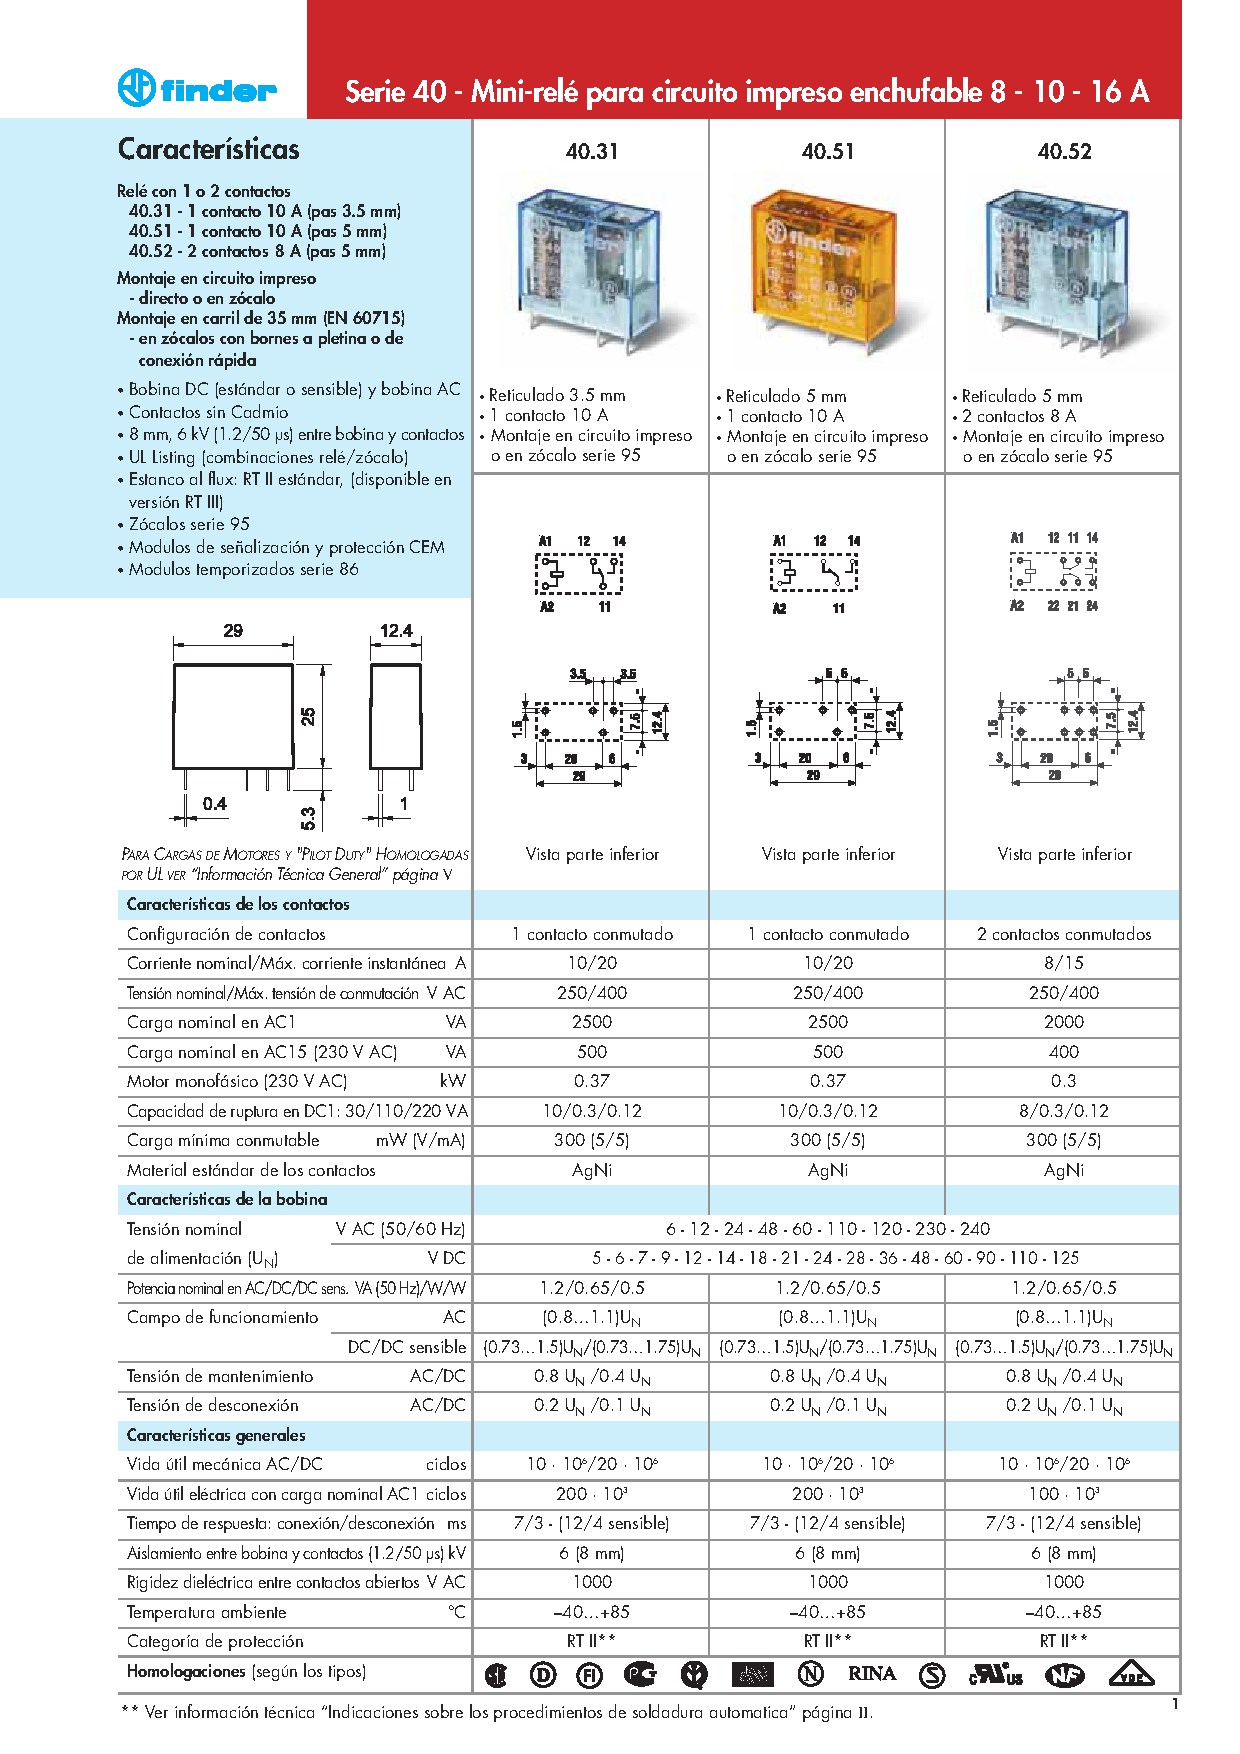
\includepdf[pages={1},scale=0.75,offset=5 -55,pagecommand={\section{Hoja técnica de relé 40.31 de 12V}\pagestyle{fancytfg}}]{./contenido/content-anexos/relay_4031_12V.pdf}

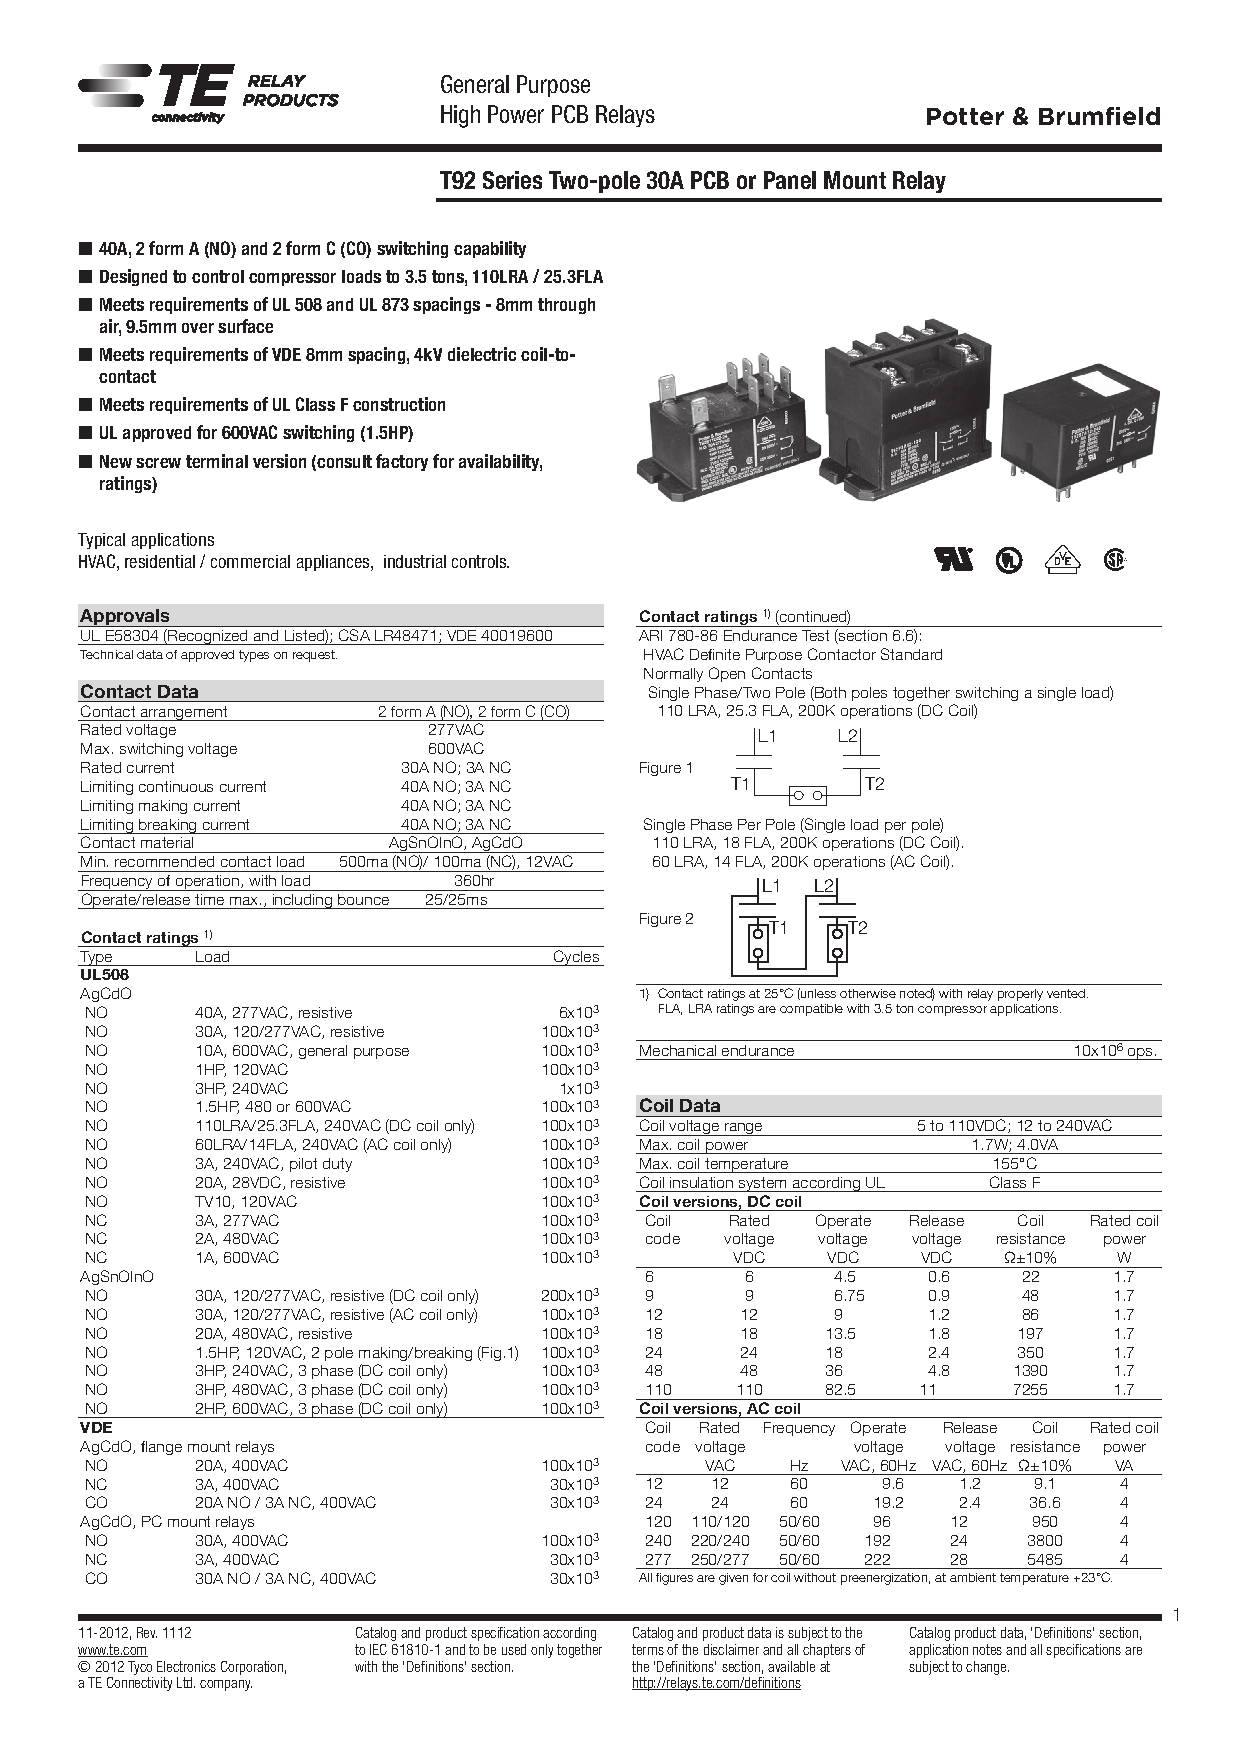
\includepdf[pages={1},scale=0.8,offset=-15 -35,pagecommand={\section{Hoja técnica de relé T92S7A12 de 240V}\pagestyle{fancytfg}}]{./contenido/content-anexos/relay_T92_240V.pdf}